\chapter{Mesterséges intelligencia betanítása és használata}
\thispagestyle{fancy}
\pagestyle{fancy}


A célom az volt, hogy a mesterséges intelligencia játéka, a lehető legjobban hasonlítson az emberi gondolkodáshoz. Az emberi agy működéséhez a legjobban 
a neurális hálózat hasonlítható, így ezt használtam én is a projektemhez. 



\section{TensorFlow}
Python nyelven terveztem elkészíteni az MI tanításához az algoritmust. Ehhez a legjobbnak a TensorFlow-t \cite{tensorflow2015-whitepaper} találtam.
A TensorFlow weboldalán ingyenesen elérhető dokumentációkból és tanító anyagokból indultam ki. 

A dokumentáció szerint, minden felhasználónak alapvetően a Keras API \cite{chollet2015keras} használatát javasolják, így hát én is azt használtam. 

\section{Tervezés}
Az elképzelésem szerint, egy Sequential, azaz szekvenciális modellt használtam. A szekvenciális modellben pontosan egyetlen egy bemeneti tensor és egyetlen egy kimeneti tensor található.

Az én esetemben a bemeneti tensor a játék jelenlegi állása volt, a kimenet pedig a következő felfordítandó kártya lett. Mivel a tensornak a típusa nem változott, pusztán az értéke, ezért nekem ez tökéletesen megfelelő volt.

A modellt be kellett tanítanom a gyűjtött adatokkal. Ehhez a legegyszerűbb az volt, ha az adataimat egy JSON fájlba összefűztem, így a scriptnek elég volt ezt az egy fájlt beolvasnia.

Minél jobban le tudtam egyszerűsíteni a bemeneti rétegem, úgy, hogy lehetőleg ne legyen benne adatvesztés, annál gyorsabban véghez tudtam vinni a tanítást. 
Ha bonyolult volt az input layer, akkor a tanulás lelassult, és számomra fontos perceket, órákat, de akár napokat is veszíthettem volna egy hibás modell esetén.

Példának okáért, tegyük fel, hogy nem transzformálom át a gyűjtött adatokat, és a játék $N$ lépésből áll. 
Mivel mind az $N$ esetben az előző $N-1$ lépést is oda kell adnom a tanító algoritmusnak, és 1.-től $N.$-ik lépésig az összes lépést meg kell tanítanom a modellnek, 
így egy $N$ lépésből álló játéknak a tanításhoz felhasznált adatmennyisége:

\begin{equation}\label{eq:1}
\frac{N(N+1)}{2} = \frac{N^2+N}{2}
\end{equation}

Látható, hogy négyzetesen nő az adatok mennyisége. Annak érdekében, hogy ezt elkerüljem, a következő ötlettel álltam elő:

A hash-függvényeket az informatikában az 1980-as évek óta alkalmazzák arra, hogy bármilyen méretű adatot rögzített hosszúságúra alakítsanak át. Gyakorlati felhasználási területük például a fájlok ellenőrzése. 
Ha két fájl tartalma teljesen megegyezik, akkor az azokból képzett hash is azonos lesz. 
Ez különösen hasznos, amikor dokumentumokat töltünk fel egy fájlszerverre, így könnyen ellenőrizhető, hogy a fájl már létezett-e a szerveren, és elkerülhető a duplikált tárolás.

A hash-függvények segítségével képes voltam minden lépést és az őt megelőző összes eddigi lépés együttesét fix hosszú bit vektorrá átalakítani, így szignifikáns mennyiségű adatmennyiséget tudtam spórolni.
Természetesen fennállt annak a lehetősége, hogy a betanított modellem nem lesz teljesen pontos, azonban ez a kockázat minden transzformációs folyamat során előfordulhat.

\begin{figure}[h]
    \centering
    \begin{adjustbox}{width=0.75\textwidth}
        \label{diagram:deepLearningModel}  
        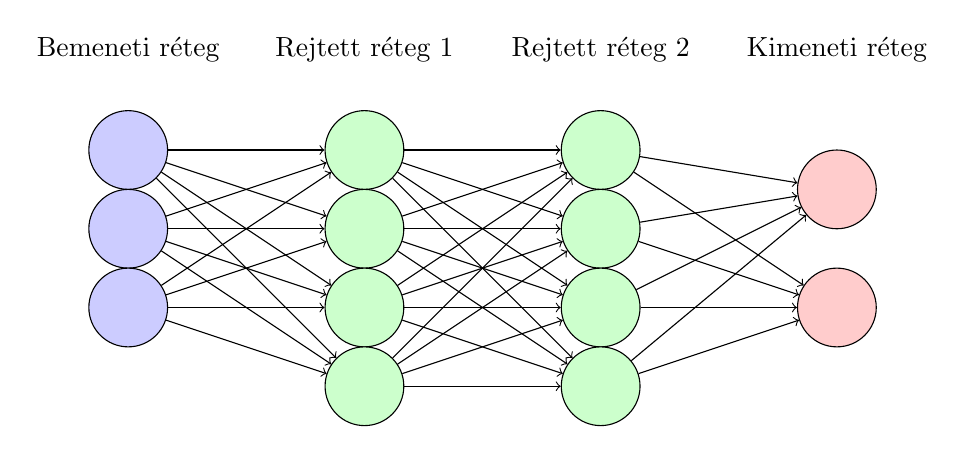
\begin{tikzpicture}[
            node distance=1.5cm and 2cm,
            input neuron/.style={circle, draw, fill=blue!20, minimum size=1cm},
            hidden neuron/.style={circle, draw, fill=green!20, minimum size=1cm},
            output neuron/.style={circle, draw, fill=red!20, minimum size=1cm},
            neuron missing/.style={draw=none, fill=none, text height=0.5cm, execute at begin node=\color{black}$\vdots$}
        ]
        
        % Input layer
        \foreach \m in {1,2,3}
            \node[input neuron] (I-\m) at (0,-\m) {};
        
        % Hidden layer 1
        \foreach \m in {1,2,3,4}
            \node[hidden neuron] (H1-\m) at (3,-\m) {};
        
        % Hidden layer 2
        \foreach \m in {1,2,3,4}
            \node[hidden neuron] (H2-\m) at (6,-\m) {};
        
        % Output layer
        \foreach \m in {1,2}
            \node[output neuron] (O-\m) at (9,-1.5*\m) {};
        
        % Connect input layer to hidden layer 1
        \foreach \i in {1,2,3}
            \foreach \j in {1,2,3,4}
                \draw[->] (I-\i) -- (H1-\j);
        
        % Connect hidden layer 1 to hidden layer 2
        \foreach \i in {1,2,3,4}
            \foreach \j in {1,2,3,4}
                \draw[->] (H1-\i) -- (H2-\j);
        
        % Connect hidden layer 2 to output layer
        \foreach \i in {1,2,3,4}
            \foreach \j in {1,2}
                \draw[->] (H2-\i) -- (O-\j);
        
        % Labels
        \node[above] at (0,0) {Bemeneti réteg};
        \node[above] at (3,0) {Rejtett réteg 1};
        \node[above] at (6,0) {Rejtett réteg 2};
        \node[above] at (9,0) {Kimeneti réteg};
        
        \end{tikzpicture}
    \end{adjustbox}
    \caption{Neurális háló, egy bemeneti, két rejtett és egy kimeneti réteggel}
\end{figure}

\section{Adatok transzformálása}

Az adatok transzformálását a program futása közben, felhasználás előtt készítettem elő. Ez azért volt hasznos, mivel a játék közben, a kész modell felhasználásakor is dinamikusan kellett az adatokat hash-függvénnyel leképeznem.

\begin{itemize}
    \item Beolvasom a JSON (\ref{code:json_allomany}. ábra) állományt. 
    \item Végigmegyek az adatokon, és létrehozok egy szöveges változót. Ez a változó tartalmazza a JSON-ban található aktuális valamint az összes előző lépést  (\ref{code:json_to_hash}. ábra). 
    \item A python hashlib csomagja segítségével ezt a változót leképezem az SHA256 függvényt használva egy hexadecimális stringgé. 
    \item A leképezett hexadecimális stringet tovább transzformálom. 
    Végigmegyek az összes karakterén, minden karakter egy hexadecimális szám. Ezen számokat leképezem egy decimális számmá, majd tovább konvertálom egy 4 bit hosszú binárissá. Ezen 4 számjegyű számokat összefűzöm egy stringgé, majd átkonvertálom, hogy egy darab 256 bitből álló NumPy tömböt kapjak, melyet fel fogok tudni használni a tanításhoz (\ref{code:hash_to_bit}. ábra). 
\end{itemize}

\begin{figure}[h]
    \center
    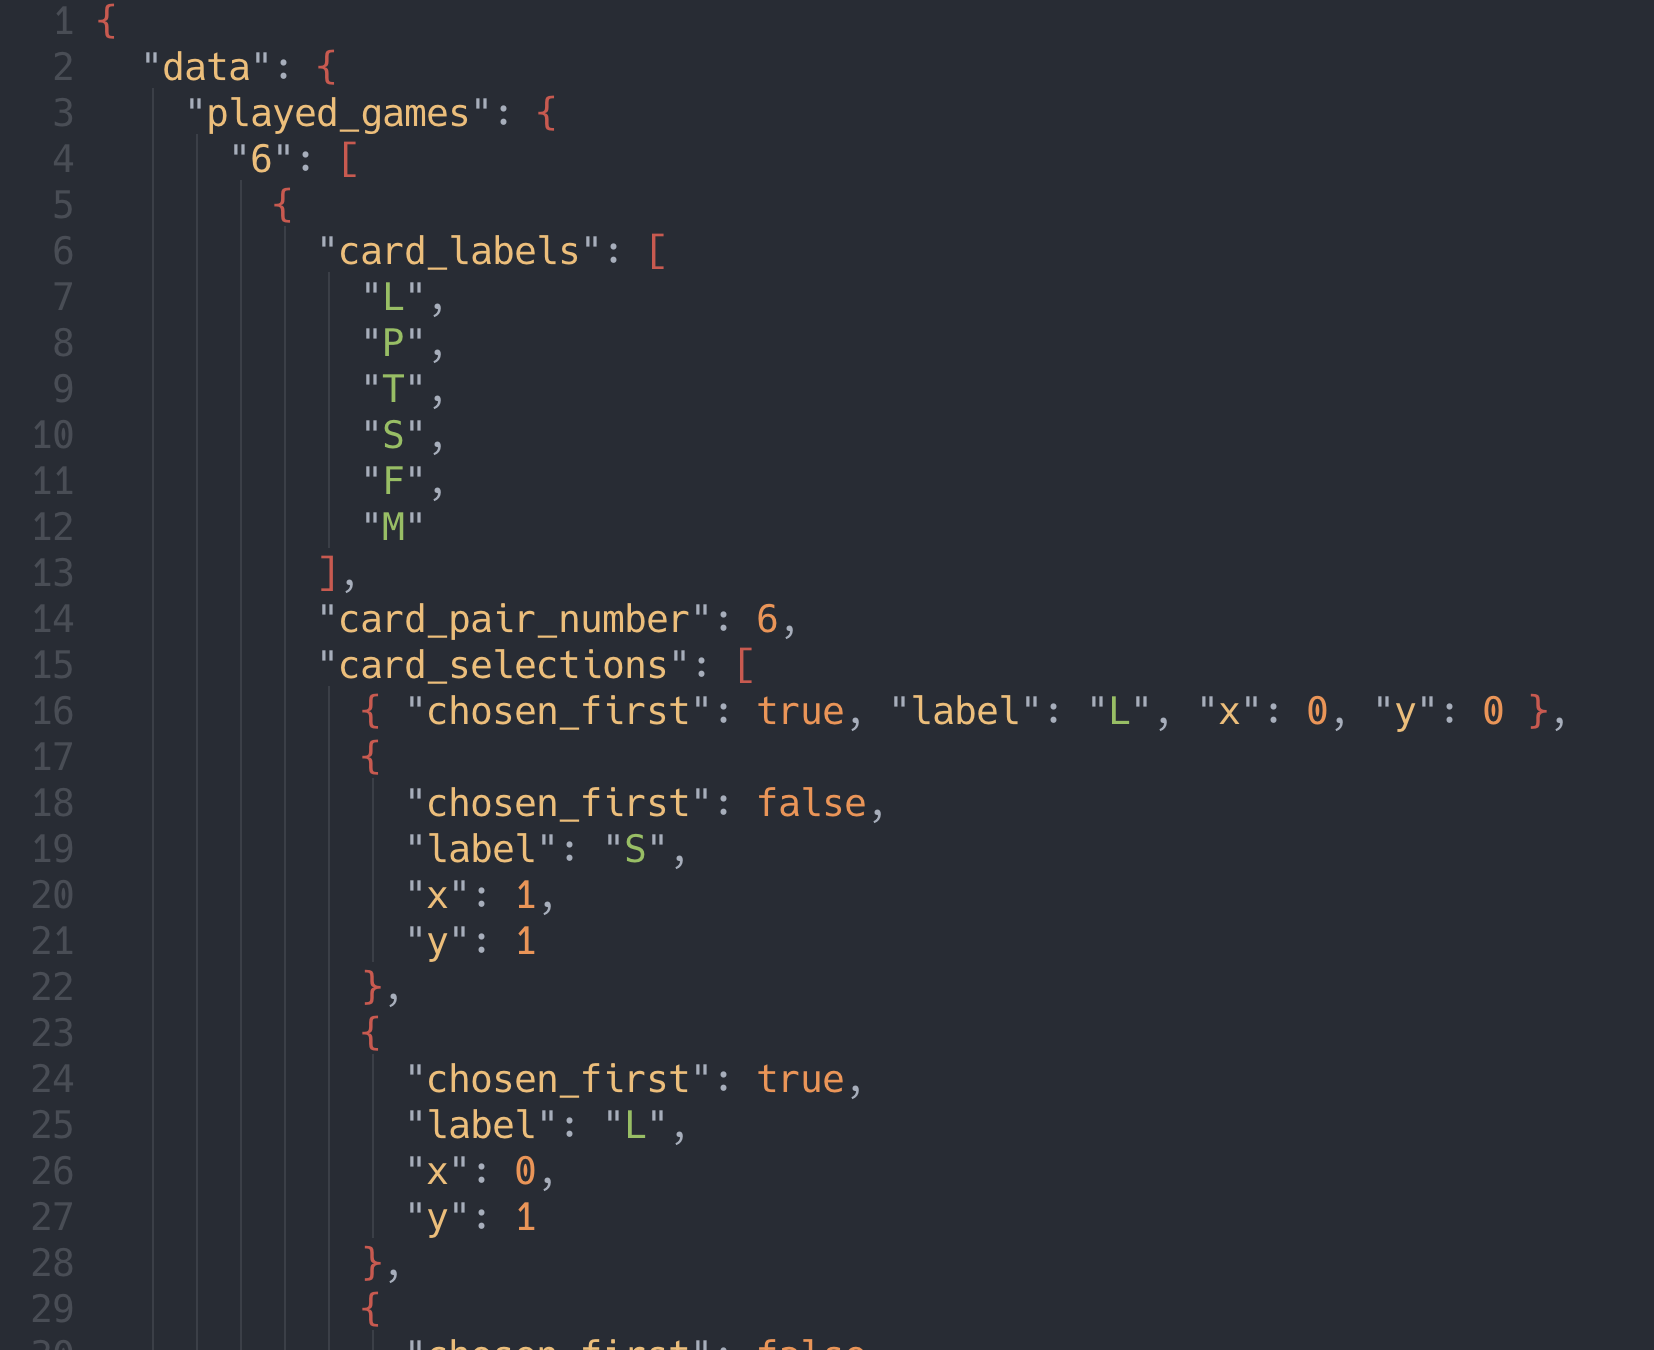
\includegraphics[width=0.60\textwidth]{img/JSON.png}
    \caption{Gyűjtött adat JSON állomány részlet.}
    \label{code:json_allomany}
\end{figure}
\begin{figure}[h]
    \center
    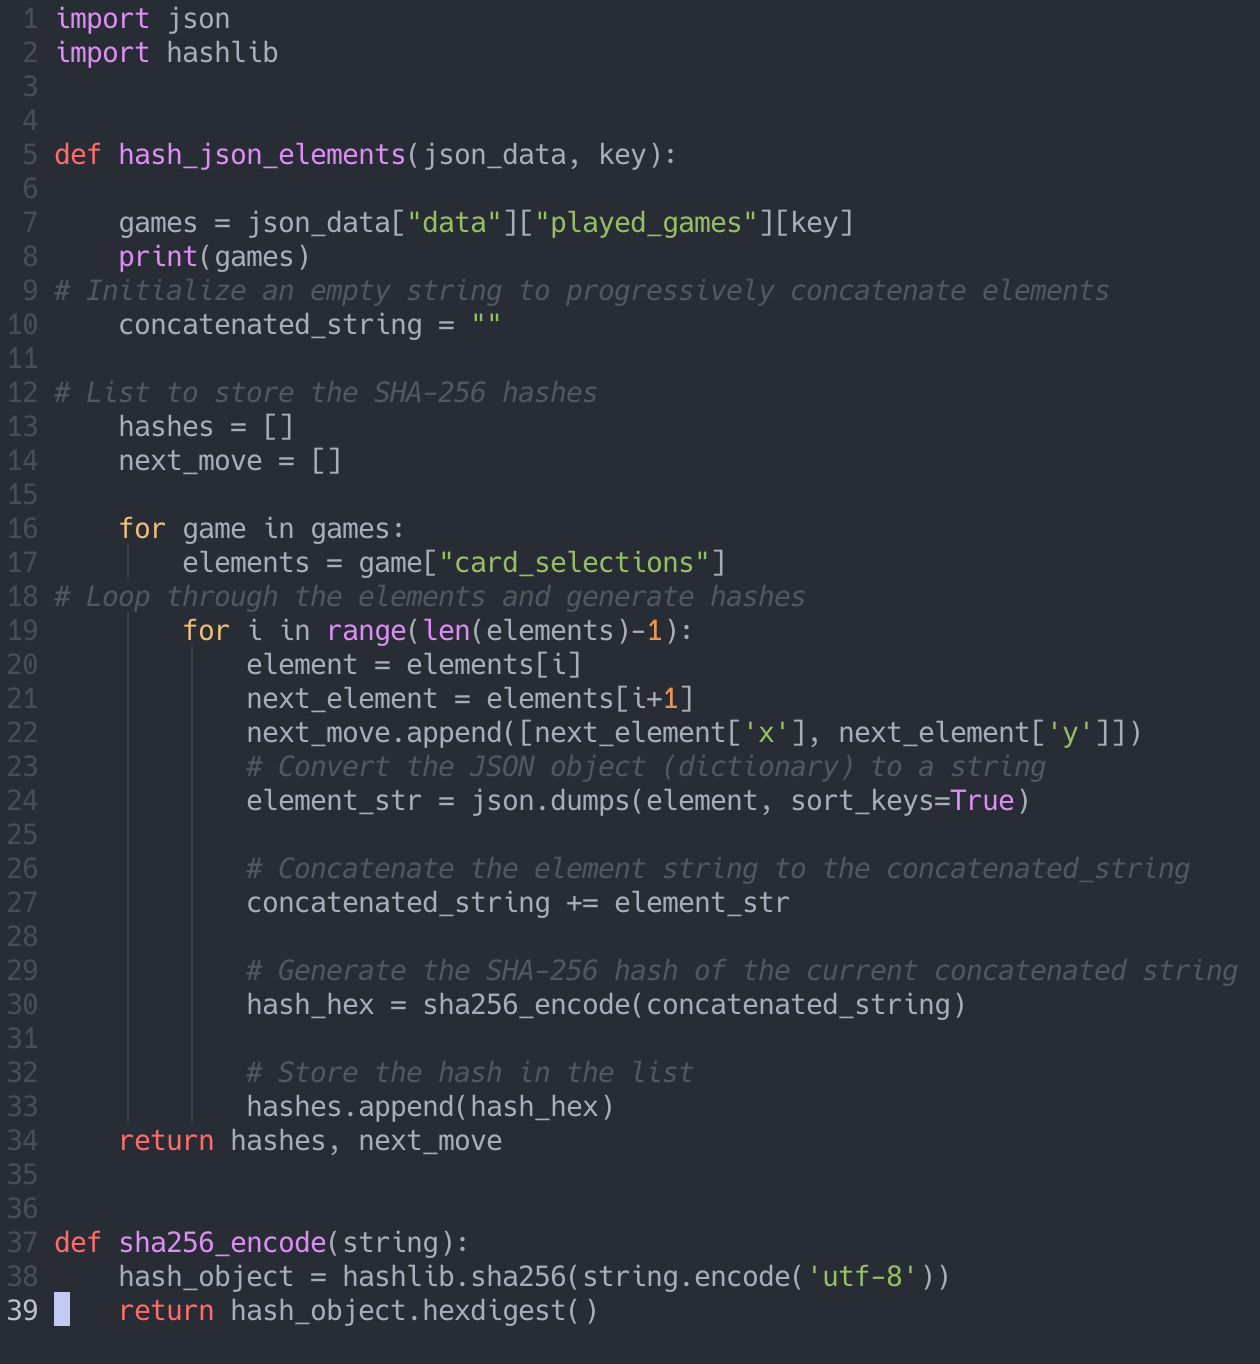
\includegraphics[width=0.60\textwidth]{img/JSON_TO_SHA256.png}
    \caption{Kód részlet, amely leképezi a \lstinline{key} által megadott játék lépéseit egy hash tömbbé. A hash-ek mellett a következő lépéseket tartalmazó tömbbel tér vissza.}
    \label{code:json_to_hash}
\end{figure}

\begin{figure}[h]
    \center
    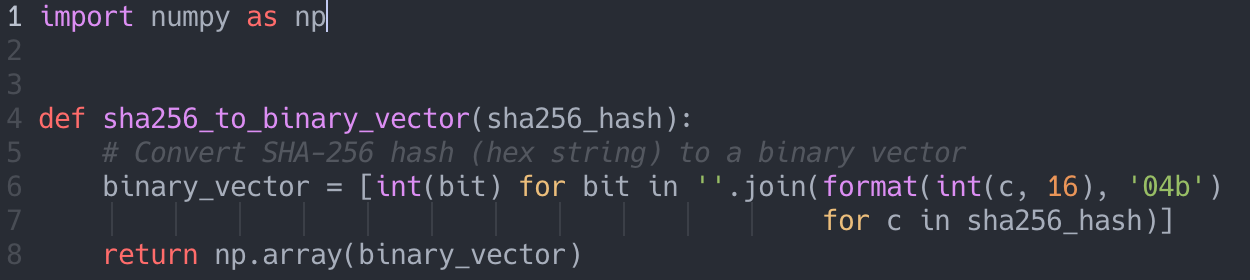
\includegraphics[width=0.60\textwidth]{img/hash_to_bit.png}
    \caption{Kód részlet. Az SHA256 hash hexadecimális string bitsorozattá konvertálása.}
    \label{code:hash_to_bit}
\end{figure}

\section{A tanító algoritmus}

\subsection{A modell elkészítése}
A TensorFlow része a Keras API, mely segítségével könnyedén és egyszerűen létre tudok hozni szekvenciális modellt (\ref{code:tensor}. ábra). A modell bemeneti rétege egy 256 nagyságú tömböt vár, melyben bitek találhatók. 

A következő két réteghez egy 128 és egy 64 neuront tartalmazó teljesen kapcsolodó (Dense) réteget használok. Dense layer azt jelenti, hogy a réteg összes neuronja kapcsolodik az előző réteg összes neuronjával. Ez a neuron típus gyarkan használt előre csatolt neurális hálóknál.
Az aktivációs függvény, amit ezekhez a rétegekhez használok, az az úgynevezett 
ReLU (Rectified Linear Unit) függvény, mely a következőképpen néz ki:
\begin{equation}\label{eq:2}
\text{ReLU}(x) = \max(0, x) 
\end{equation}

ami azt jelenti, hogy ha bemeneti érték, vagyis $x$ pozitív, akkor $x$-et adja vissza, ha negatív, akkor 0-t. 


\begin{figure}[h]
    \center
    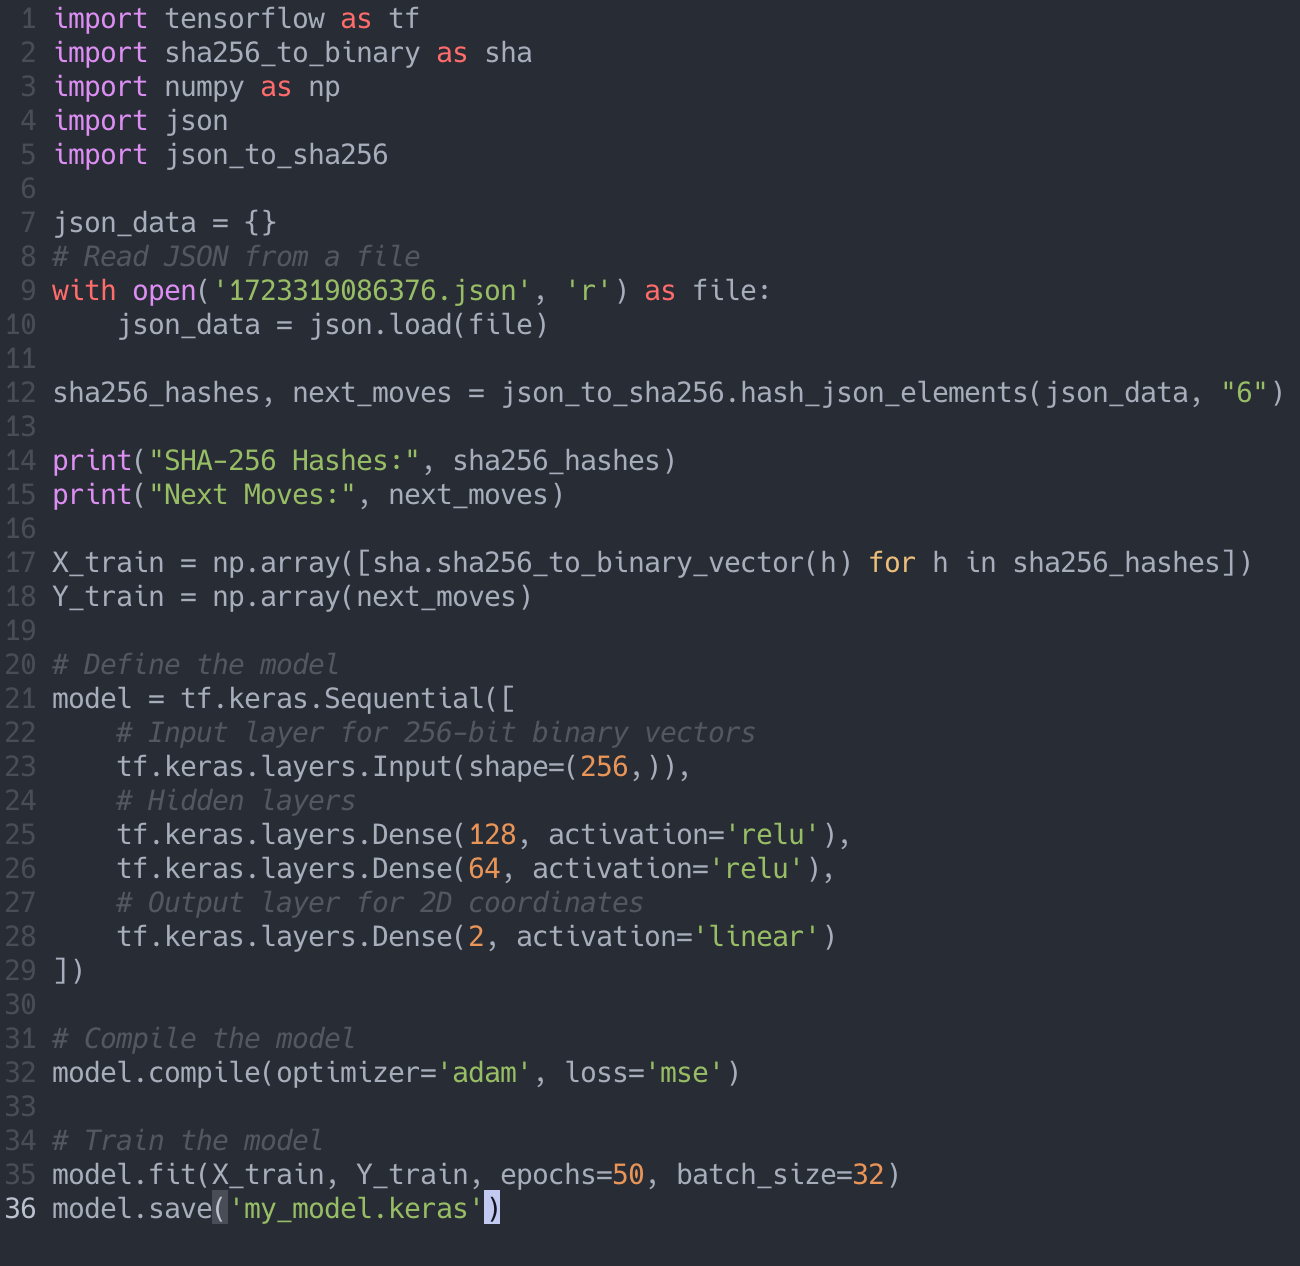
\includegraphics[width=0.75\textwidth]{img/Tensor.png}
    \caption{Kód részlet. A tanító algoritmus}
    \label{code:tensor}
\end{figure}

Az aktivációs függvények célja, hogy nemlinearitást vigyenek a modellbe, lehetővé téve a bonyolult mintázatok felismerését az adatokban. 
Ha nem használnánk aktivációs függvényeket, a modell kimenete csak az inputok egyszerű lineáris kombinációja lenne, ami korlátozná a modell képességeit a komplex kapcsolatok megragadásában.
A ReLU ezért olyan népszerű a mélytanulásban, mert csökkenti gradiensek eltűnésének problémáját, így gyorsabb tanulást és jobb teljesítményt tesz lehetővé.

A kimeneti réteghez egy 2 neuronból álló lineáris aktivációs függvénnyel ellátott réteget használok. A lineáris aktivációs függvény azt jelenti, hogy a neuron kimenete az inputok lineáris kombinációja, ami lényegében nem végez átalakítást. Matematikailag ez így írható le:
\begin{equation}\label{eq:3}
\text{kimenet} = \text{bemenet} \cdot \text{súlyok} + \text{eltolás}
\end{equation}
    

A linear aktivációs függvény használatakor a réteg lényegében nem változtatja meg a bemeneti értékeket, csak a súlyokat és az eltolást alkalmazza.

A modell lefordításához, az $adam$ optimizálót használom, valamint az mse (mean squared error) vagyis az átlagos négyzetes hiba módszert. 
Ez az összeállítás biztosítja, hogy a modell hatékonyan és gyorsan tudjon tanulni a bemeneti adatokból, minimalizálva az előrejelzések és a valós értékek közötti hibát.

\subsection{A modell betanítása}
A modell betanításához szükségem van a hash tömbbé alakított adatokra, valamint ötven tanítási cikluson keresztül az aktuális következő lépések tömbjére. 
Minden edzési lépés során a modell harminckét mintát tartalmazó adatcsomagot dolgoz fel.
Ez a folyamat lehetővé teszi a modell számára, hogy fokozatosan javítson a teljesítményén az adatok ismételt bemutatása és a súlyok frissítése révén. 

A betanított modellt egy \lstinline{my_model.keras} fájlba mentettem le, így könnyen tudtam használni, a játék futtatásakor. 

\section{Modell használata}

\subsection{Python Script API a modell használatához}

Ahhoz, hogy a modellt használni tudjam, egy API-t kellett írnom. Mivel a tesztadatokat is HTTP-kérés segítségével küldtem el, így logikusnak találtam, hogy ezt a megoldást használjam itt is. 

A folyamatot a \ref{code:modell_hasznalata}. ábrával szemléltetem.

\begin{figure}[h]
    \center
    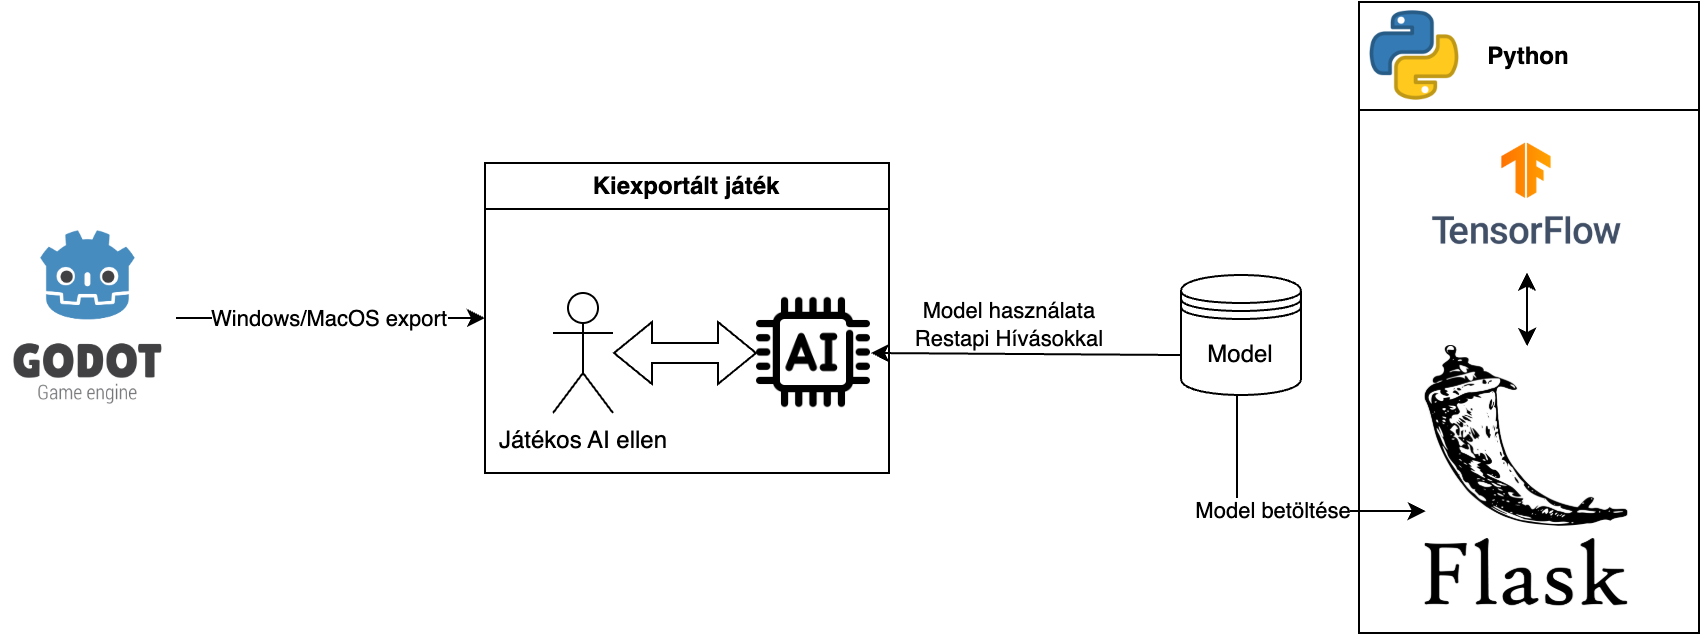
\includegraphics[width=\textwidth]{img/kiexportalt.drawio.png}
    \caption{Diagram. A modell használata.}
    \label{code:modell_hasznalata}
\end{figure}


A Flask használatával készítettem egy webalkalmazást (\ref{code:use_model}. ábra), melynek egyetlen belépési pontja van, a \lstinline{/predict}. A Memória játék ide küldi a \lstinline{POST} HTTP kérését, mely tartalmazza a játék aktuális állását. 
Vagyis az aktuális és az összes eddigi lépést.




\begin{figure}[h]
    \center
    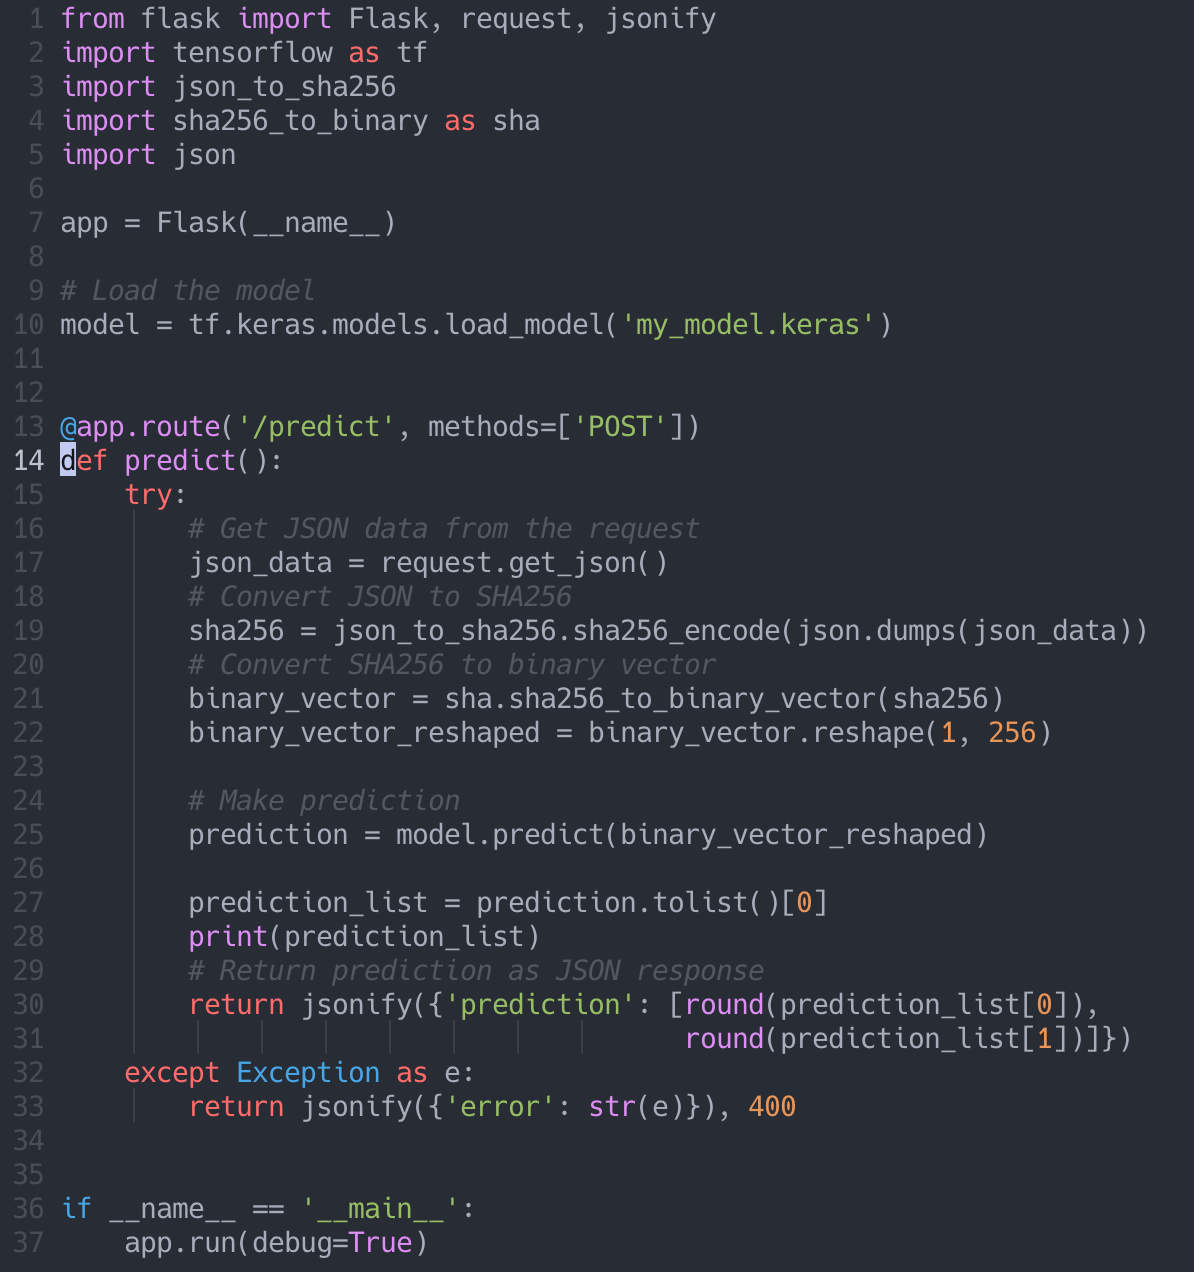
\includegraphics[width=0.75\textwidth]{img/use_model.png}
    \caption{Kód részlet. A modellt használó API}
    \label{code:use_model}
\end{figure}

\subsection{API használata}

Az API indításkor betölti a \lstinline{my_model.keras} fájlból a betanított modellünket, ez percekig is eltart, majd várja a fogadó kéréseket. 
Amikor egy kérés érkezik, a fogadott JSON adatra ráfuttatjuk a már korábban használt SHA256 konvertáló scriptet (\ref{code:json_to_hash}).
Az így kapott 256 hosszú bitsorozattal csinálunk egy "jóslást", vagyis használjuk a modellnek a predict függvényét. Ebből a jóslatból visszakapunk egy két elemű vektort, melynek elemei nem egész számok.

Mivel két pozitív egész számra, azaz koordinátára van szükségünk, a kapott értékeket kerekítjük, majd HTTP-válaszként visszaküldjük a két egész számot.
\subsection{Játék kódjában való változtatások}

A játékot, ahhoz hogy működjön a mesterséges inteligenciával, először át kellett alakítanom, hogy minden lépésem után az MI következzen. A változtatás egyszerű volt: egy változóba tárolom, hogy a játékos, vagy az MI köre van soron, és minden pár fordítása után cserélem. 

Ahhoz, hogy az MI is tudjon kártyát választani, készítettem egy \lstinline{get_ai_cards} függvényt (\ref{code:get_ai_card}. ábra). A függvény meghívja a \lstinline{\prediction} végpontot, a \lstinline{HttpClient} segítségével.
A visszakapott koordinátákból kiválasztja a kártyát az asztalon. 
Ha ez a kártya nem elérhető, mert már levették az asztalról, vagy a koordináták nem létező kártyára mutatnak, akkor a legelső elérhető kártyát fogja választani a mesterséges intelligencia. 

\begin{figure}[H]
    \centering
    \begin{lstlisting}[language=GDScript]
func get_ai_cards():
        var output;
        waiting_for_card=true;
        if data.card_selections:
            output = HttpClient.post_JSON_tensor(data.card_selections);
            waiting_for_card=false
            if output:
                var coord_x:int=output["prediction"][0]
                var coord_y:int=output["prediction"][1]
                var Card=cards[0];
                for c in cards:
                    if c.table_x==coord_x && c.table_y==coord_y:
                        Card=c
                return Card
    \end{lstlisting}
    \caption{Kód részlet: Az MI kártya választó függvénye GDScript-ben.}
    \label{code:get_ai_card}
\end{figure}
